\documentclass[tikz,border=2pt]{standalone}
\usepackage{newtxtext,newtxmath}
\usetikzlibrary{decorations.pathreplacing,arrows.meta,calc}
\definecolor{P1}{HTML}{3B6FB6}
\definecolor{P2}{HTML}{2A9D8F}
\definecolor{P3}{HTML}{7FB069}
\definecolor{P4}{HTML}{E2B13C}
\definecolor{P5}{HTML}{E07A3F}
\definecolor{A}{HTML}{8A8A8A}
\definecolor{dark}{HTML}{8B1E3F}
\definecolor{ground}{HTML}{ECEAE6}
\definecolor{edge}{HTML}{4A4A4A}
\newcommand{\br}{0.12}
\newcommand{\ball}[2]{\fill[#1, draw=#1!60!black, line width=0.4pt] #2 circle (\br);
  \fill[white, opacity=0.55] ($#2+(-0.04,0.045)$) circle (0.028);}
\newcommand{\ghost}[3]{\fill[#1, opacity=#2] #3 circle (\br);}
\newcommand{\assistant}[1]{\fill[white, draw=black, line width=0.6pt] #1 circle (\br);
  \node[font=\fontsize{5.5}{6}\selectfont\bfseries, inner sep=0] at #1 {A};}
% Landscapes (EB: base, EC: after collapse) and ball rest positions, precomputed
\def\EB{1.6+1.4*((\x-2.5)/2.5)^24-0.8*(exp(-(min(((\x-0.9)/0.2)^2,30))^2)+exp(-(min(((\x-1.5)/0.2)^2,30))^2)+exp(-(min(((\x-2.1)/0.2)^2,30))^2)+exp(-(min(((\x-2.7)/0.2)^2,30))^2)+exp(-(min(((\x-3.3)/0.2)^2,30))^2)+exp(-(min(((\x-3.9)/0.2)^2,30))^2)+exp(-(min(((\x-4.5)/0.2)^2,30))^2))}
\def\EC{1.6+1.4*((\x-2.5)/2.5)^24-0.72*exp(-((\x-0.42)^2)/0.2592)-0.85*exp(-((\x-4.55)^2)/0.3528)-0.32*exp(-((\x-3.0)^2)/0.0512)}
\def\BALLSA{
  \ball{P1}{(1.500,0.920)}
  \ball{P2}{(2.100,0.920)}
  \ball{P3}{(2.700,0.920)}
  \ball{P4}{(3.300,0.920)}
  \ball{P5}{(3.900,0.920)}
  \assistant{(4.500,0.943)}}
\def\BALLSB{
  \ball{P1}{(1.500,0.920)}
  \ball{P2}{(2.100,0.920)}
  \ball{P3}{(2.700,0.920)}
  \ball{P4}{(3.300,0.920)}
  \ball{P5}{(3.900,0.920)}
  \assistant{(0.900,0.920)}}
\def\BALLSC{
  \ghost{P4}{0.16}{(0.280,1.346)}
  \ghost{P4}{0.28}{(0.280,1.346)}
  \ghost{P4}{0.28}{(0.440,1.016)}
  \ghost{P4}{0.16}{(0.540,1.074)}
  \ghost{P2}{0.16}{(0.400,1.051)}
  \ghost{P2}{0.28}{(0.500,1.040)}
  \ghost{P2}{0.28}{(0.700,1.255)}
  \ghost{P2}{0.16}{(0.800,1.372)}
  \ghost{P1}{0.16}{(2.800,1.621)}
  \ghost{P1}{0.28}{(2.900,1.521)}
  \ghost{P1}{0.28}{(3.100,1.517)}
  \ghost{P1}{0.16}{(3.200,1.612)}
  \ghost{P5}{0.16}{(4.010,1.404)}
  \ghost{P5}{0.28}{(4.110,1.296)}
  \ghost{P5}{0.28}{(4.310,1.055)}
  \ghost{P5}{0.16}{(4.410,0.949)}
  \ghost{P3}{0.16}{(4.270,1.103)}
  \ghost{P3}{0.28}{(4.370,0.989)}
  \ghost{P3}{0.28}{(4.570,0.901)}
  \ghost{P3}{0.16}{(4.670,1.070)}
  \ghost{A}{0.16}{(4.520,0.881)}
  \ghost{A}{0.28}{(4.620,0.964)}
  \ghost{A}{0.28}{(4.760,1.417)}
  \ghost{A}{0.16}{(4.760,1.417)}
  \ball{P4}{(0.340,1.160)}
  \ball{P2}{(0.600,1.136)}
  \ball{P1}{(3.000,1.407)}
  \ball{P5}{(4.210,1.176)}
  \ball{P3}{(4.470,0.902)}
  \assistant{(4.720,1.231)}}
% landscape: ground fill + outline
\newcommand{\terrain}[1]{%
  \fill[ground] (0,0.55) -- plot[domain=0:5,samples=400] (\x,{#1}) -- (5,0.55) -- cycle;
  \draw[edge, line width=0.8pt] plot[domain=0:5,samples=400] (\x,{#1});
  \draw[edge!70, line width=0.4pt] (0,0.55) -- (5,0.55);
  \foreach \t in {0,...,5} {\draw[edge!70, line width=0.4pt] (\t,0.55) -- (\t,0.48);
    \node[font=\scriptsize, text=edge, anchor=north, inner sep=1.5pt] at (\t,0.48) {\t};}
  \node[font=\scriptsize, text=edge, anchor=north] at (2.5,0.18) {Harm/Care rating};}
\begin{document}
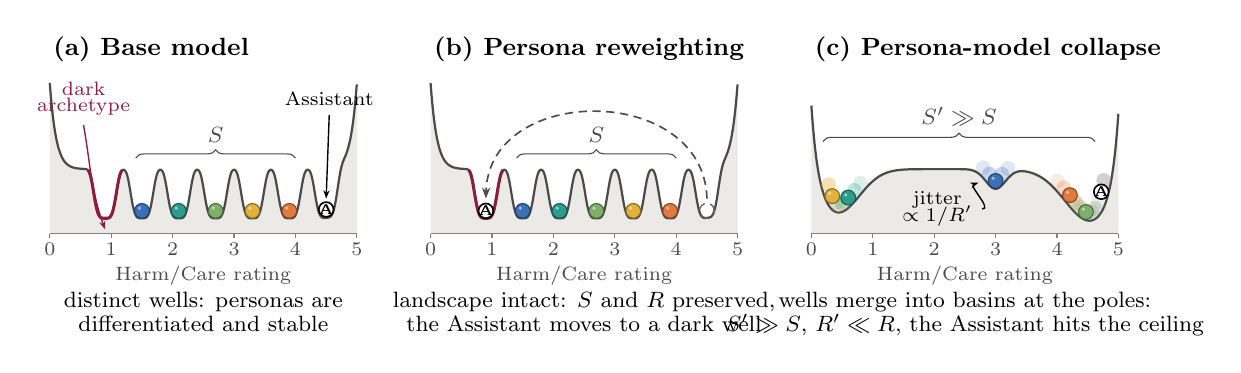
\begin{tikzpicture}[x=0.78cm,y=0.78cm]
% ---------------- (a) base
\begin{scope}
  \terrain{\EB}
  \draw[dark, line width=1.1pt] plot[domain=0.62:1.18,samples=80] (\x,{\EB});
  \BALLSA
  \node[font=\footnotesize, align=center, anchor=north] at (2.5,-0.25) {distinct wells: personas are\\[-1pt]differentiated and stable};
  \node[font=\small\bfseries, anchor=west] at (-0.1,3.55) {(a) Base model};
  \draw[decorate, decoration={brace, amplitude=3pt}, edge] (1.4,1.78) -- node[above=2pt, font=\footnotesize] {$S$} (4.0,1.78);
  \node[font=\scriptsize, text=dark, align=center] (dk) at (0.55,2.75) {dark\\[-2pt]archetype};
  \draw[dark, -{Stealth[length=3pt]}, line width=0.5pt] (dk.south) to[out=-80,in=110] (0.9,0.62);
  \node[font=\scriptsize, align=center] (as) at (4.55,2.75) {Assistant};
  \draw[-{Stealth[length=3pt]}, line width=0.5pt] (as.south) -- (4.5,1.12);
\end{scope}
% ---------------- (b) reweighting
\begin{scope}[xshift=6.2*0.78cm]
  \terrain{\EB}
  \draw[dark, line width=1.1pt] plot[domain=0.62:1.18,samples=80] (\x,{\EB});
  \draw[black!60, densely dashed, line width=0.5pt] (4.5,0.923) circle (\br);
  \BALLSB
  \node[font=\footnotesize, align=center, anchor=north] at (2.5,-0.25) {landscape intact: $S$ and $R$ preserved,\\[-1pt]the Assistant moves to a dark well};
  \draw[-{Stealth[length=4pt]}, line width=0.6pt, black!70, densely dashed] (4.5,1.12) .. controls (4.45,3.0) and (0.95,3.0) .. (0.9,1.12);
  \node[font=\small\bfseries, anchor=west] at (-0.1,3.55) {(b) Persona reweighting};
  \draw[decorate, decoration={brace, amplitude=3pt}, edge] (1.4,1.78) -- node[above=2pt, font=\footnotesize] {$S$} (4.0,1.78);
\end{scope}
% ---------------- (c) collapse
\begin{scope}[xshift=12.4*0.78cm]
  \terrain{\EC}
  \BALLSC
  \node[font=\footnotesize, align=center, anchor=north] at (2.5,-0.25) {wells merge into basins at the poles:\\[-1pt]$S'\gg S$, $R'\ll R$, the Assistant hits the ceiling};
  \node[font=\scriptsize, align=center] (jt) at (2.05,0.95) {jitter\\[-2pt]$\propto 1/R'$};
  \draw[-{Stealth[length=3pt]}, line width=0.5pt] (jt.east) to[out=0,in=200] (2.72,1.38);
  \node[font=\small\bfseries, anchor=west] at (-0.1,3.55) {(c) Persona-model collapse};
  \draw[decorate, decoration={brace, amplitude=3pt}, edge] (0.19,2.05) -- node[above=2pt, font=\footnotesize] {$S'\gg S$} (4.62,2.05);
\end{scope}
\end{tikzpicture}
\end{document}
